\documentclass[11pt, a4paper]{article}

\usepackage{tikz}
\usetikzlibrary{shapes,arrows}
\usepackage{amsmath}
\usepackage{placeins}
\usepackage{amssymb}

\begin{document}

\title{PRINCIPAL COMPONENT ANALYSIS}
\date{}
\maketitle

Principal Component Analysis (PCA) is non-parametric approach to transform a set of observations - of possibly correlated variables - into another set of values defined by a calculated set of new orthogonal uncorrelated variables called principal components. 

\section{Example}

Consider the following set of four observations in two dimesions,

\begin{figure}[htbp]
	\centering
	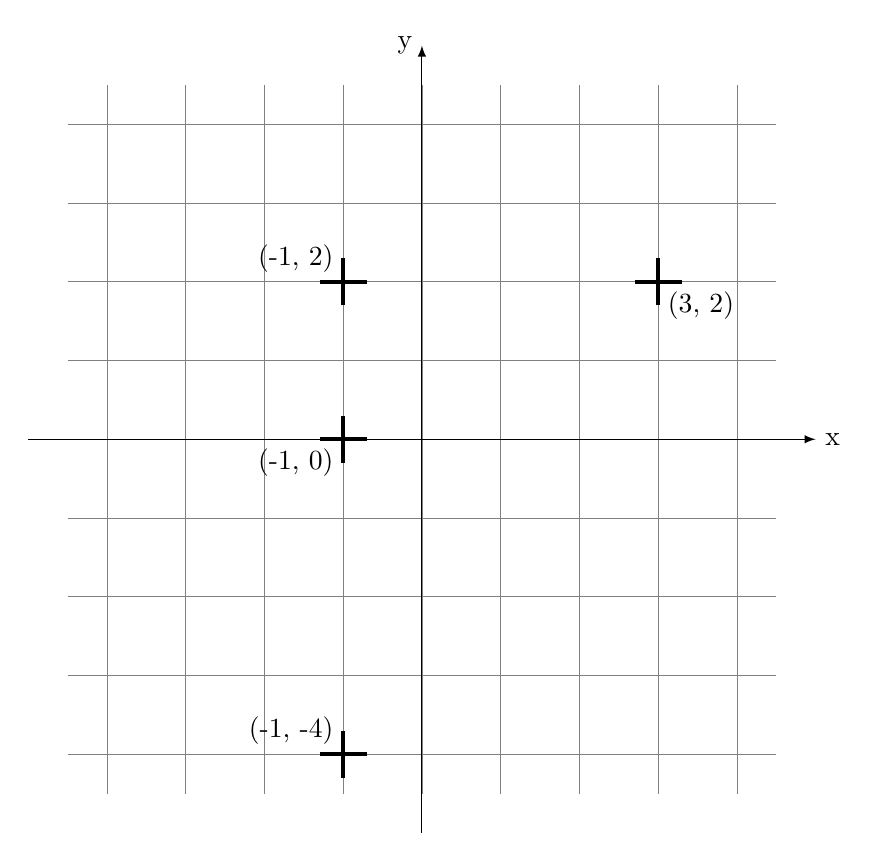
\begin{tikzpicture}
		\tikzstyle {point line} = [line width=0.15em]
		\tikzstyle {margin} = [dashed]
				
		\draw[step=1.0, gray, very thin] (-4.5, -4.5) grid (4.5, 4.5);
								    
		\draw[-latex] (-5,0) -- (5,0) node[right]{x};
		\draw[-latex] (0,-5) -- (0,5) node[left]{y};	
						
		\draw[point line] (2.7, 2) -- (3.3, 2);	
		\draw[point line] (3, 1.7) -- (3, 2.3);
		\draw (3, 2) node [below right] {(3, 2)};    	
				
		\draw[point line] (-1.3, 0) -- (-0.7, 0);	
		\draw[point line] (-1, -0.3) -- (-1, 0.3);	
		\draw (-1, 0) node [below left] {(-1, 0)};   
				
		\draw[point line] (-1.3, 2) -- (-0.7, 2);	
		\draw[point line] (-1, 1.7) -- (-1, 2.3);	
		\draw (-1, 2) node [above left] {(-1, 2)};   
				
		\draw[point line] (-1.3, -4) -- (-0.7, -4);	
		\draw[point line] (-1, -4.3) -- (-1, -3.7);	
		\draw (-1, -4) node [above left] {(-1, -4)};   
					   		
	\end{tikzpicture}
\end{figure}

To see how PCA alters the representation of this tiny dataset, the dataset is first written in matrix form as follows,

\begin{align*}
	X & = \begin{pmatrix} 3 & -1 & -1 & -1 \\
	2 & 0 & 2 & -4  
	\end{pmatrix}
\end{align*}

The x-axis intercepts are represented by the first row of this matrix while y-axis intercepts are represented by the second row.
This matrix can be thought of as a representation composed of two random variables x and y. The variances of these variables and their covariance are useful quantities to describe the structure of the dataset.

\begin{align*}
	Var(x)    & = \frac{1}{N} \sum\limits_{i = 1}^N (x_i - \bar{x})^2              \\
	          & = \frac{1}{4} \sum\limits_{i = 1}^4 (x_i - 0)^2                    \\
	          & = \frac{1}{4} |x|^2                                                \\
	          & = \frac{3^2 + (-1)^ 2 + (-1)^2 + (-1)^2}{4}                        \\
	          & = 3                                                                \\
	Var(y)    & = \frac{1}{4} \sum\limits_{i = 1}^4 (y_i - 0)^2                    \\
	          & = \frac{1}{4} |y|^2                                                \\
	          & = \frac{2^2 + 0^ 2 + 2^2 + (-4)^2}{4}                              \\           
	          & = 6                                                                \\
	Cov(x, y) & = \frac{1}{N} \sum\limits_{i = 1}^N (x_i - \bar{x})(y_i - \bar{y}) \\
	          & = \frac{1}{4} \sum\limits_{i = 1}^4 (x_i - 0)(y_i - 0)             \\  
	          & = \frac{1}{4} \vec{x}.\vec{y}                                      \\
	          & = \frac{3*2 + (-1)*0 + (-1)*2 + (-1)*(-4)}{4}                      \\
	          & = 2                                                                
\end{align*}

Note that the mean of both the vectors is zero in the dataset. This is a necessary precondition for PCA, the reason for this constraint will become apparent in later sections. Next, these variances and covariance are arranged in a matrix as follows.

\begin{align*}
	\sum & = \begin{pmatrix} Var(x) & Cov(x, y) \\
	Cov(x, y) & Var(y) \\ 
	\end{pmatrix} \\
	     & = \begin{pmatrix} 3      & 2         \\
	2 & 6 \\ 
	\end{pmatrix}           
\end{align*}

Due to zero mean constraint, the following also holds true,

\begin{align*}
	\sum = \frac{1}{N} XX^T \\
\end{align*}

Now eigenvalues and eigenvectors of $\sum$ are calculated.

\begin{align*}
	\sum \phi              & = \lambda \phi \\
	(\sum - \lambda I)\phi & = 0            
\end{align*}

$(\sum - \lambda I)$ must be singular if eigenvectors are non-zero. Hence,

\begin{align*}
	\begin{vmatrix} 3 - \lambda & 2           \\
	2                           & 6 - \lambda \\ 
	\end{vmatrix}               & = 0         \\
	(3 - \lambda)(6 - \lambda)  & = 4         \\	                
\end{align*}

This gives eigenvalues $\lambda = 2, 7$ and eignevectors $\phi = (\frac{-2}{\sqrt{5}}, \frac{1}{\sqrt{5}}), (\frac{1}{\sqrt{5}}, \frac{2}{\sqrt{5}}) $ respectively. Now the eigenvectors are arranged as rows in a matrix in order of their corresponding eigenvalue. 


\begin{align*}
	P & = \begin{pmatrix} \frac{1}{\sqrt{5}}   & \frac{2}{\sqrt{5}} \\
	\frac{-2}{\sqrt{5}} & \frac{1}{\sqrt{5}} \\ 
	\end{pmatrix}  \\
	  & = \frac{1}{\sqrt{5}} \begin{pmatrix} 1 & 2                  \\
	-2 & 1\\ 
	\end{pmatrix}	                
\end{align*}

Now the transformed dataset Y is calculated simply as product of P and X.

\begin{align*}
	P &= \frac{1}{\sqrt{5}} \begin{pmatrix} 1 & 2 \\
	-2 & 1\\ 
	\end{pmatrix} \begin{pmatrix} 3 & -1 & -1 & -1 \\
	2 & 0 & 2 & -4  
	\end{pmatrix} \\ 
	  & = \frac{1}{\sqrt{5}} \begin{pmatrix} 7 & -1 & 3 & -9 \\
	-4 & 2 & 4 & -2  
	\end{pmatrix}
\end{align*}

To visualize the result, Y is plotted on a graph,

\FloatBarrier\clearpage
\begin{figure}[htbp]
	\centering
	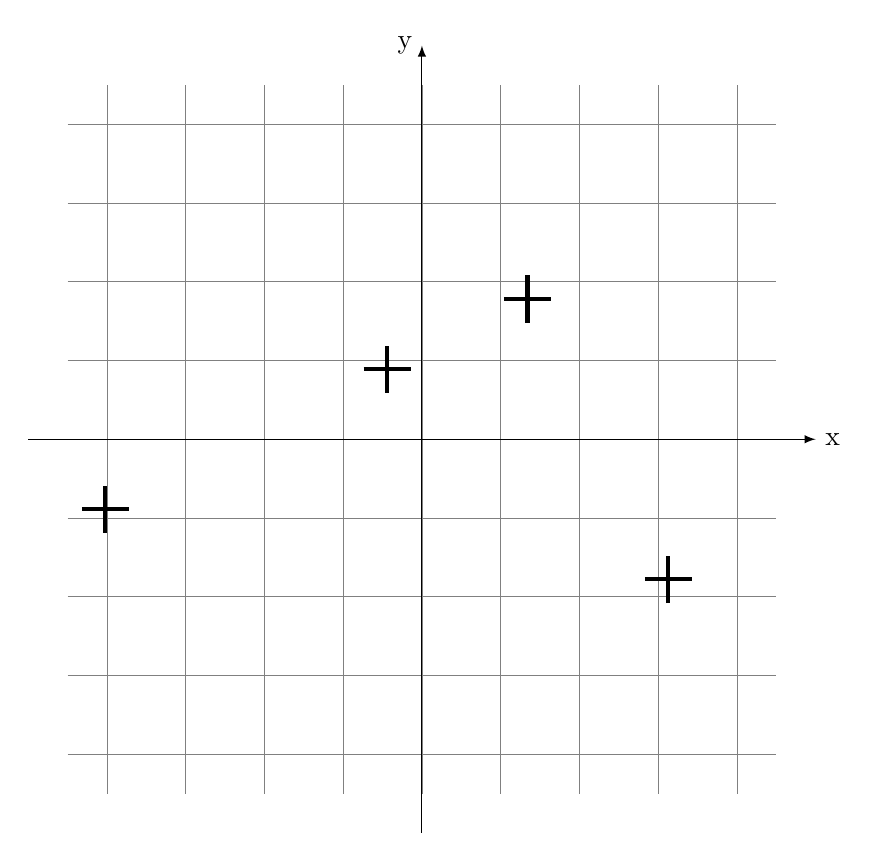
\begin{tikzpicture}
		\tikzstyle {point line} = [line width=0.15em]
		\tikzstyle {margin} = [dashed]
				
		\draw[step=1.0, gray, very thin] (-4.5, -4.5) grid (4.5, 4.5);
								    
		\draw[-latex] (-5,0) -- (5,0) node[right]{x};
		\draw[-latex] (0,-5) -- (0,5) node[left]{y};	
						
		\draw[point line] (2.83, -1.78) -- (3.43, -1.78);	
		\draw[point line] (3.13, -2.08) -- (3.13, -1.48);
		\draw (3.13, -1.78) node [below right] {};    	
				
		\draw[point line] (-0.74, 0.89) -- (-0.14, 0.89);	
		\draw[point line] (-0.44, 0.59) -- (-0.44, 1.19);	
		\draw (-0.44, 0.89) node [below left] {};   
				
		\draw[point line] (1.04, 1.78) -- (1.64, 1.78);	
		\draw[point line] (1.34, 1.48) -- (1.34, 2.08);	
		\draw (1.34, 1.78) node [above left] {};   
				
		\draw[point line] (-4.32 , -0.89) -- (-3.72 , -0.89);	
		\draw[point line] (-4.02, -1.19) -- (-4.02,-0.59 );	
		\draw (-4.02, -0.89) node [above left] {};   
					   		
	\end{tikzpicture}
\end{figure}

Visually, the points on the transformed graph arise due to a change of axes from the original axes to the axes defined by the eigenvectors of $\sum$. To see why this choice of axes was made, the variance covariance matrix of the transformed data is calculated.

\begin{align*}
	\sum_y &= \frac{1}{N} YY^T \\
	  & = \frac{1}{4} \frac{1}{\sqrt{5}} \begin{pmatrix} 7 & -1 & 3 & -9 \\
	-4 & 2 & 4 & -2  
	\end{pmatrix} \frac{1}{\sqrt{5}}  \begin{pmatrix} 7 & -4 \\
	-1 & 2 \\
	3 & 4 \\
	-9 & -2 \\   
	\end{pmatrix} \\
	&=  \frac{1}{20} \begin{pmatrix} 140 & 0 \\
	0 & 40 
	\end{pmatrix} \\
	&= \begin{pmatrix} 7 & 0 \\
	0 & 2 
	\end{pmatrix}          
\end{align*}

Two notes - the variance covariance matrix of transformed data is diagonalized meaning there is no correlation between the new variables and the variance values i.e. the diagonal terms are equal to the eigenvalues. 

This is the central point of PCA: it gives you a transformation of variables which are uncorrelated and you are free to choose a subset of these variables depending on the tradeoff between smaller number of dimensions vs loss in variance. In practice, a large chunk of calculated variables in the bottom right part of the diagonal are near zero in their variance and thus are ignored resulting in dimensionality reduction.

\end{document}
